\documentclass[journal,twoside,web]{ieeecolor}
\usepackage{generic}
\usepackage{amsmath,amssymb,amsfonts}
\usepackage{booktabs}
\usepackage{array}
\usepackage{graphicx}
\usepackage{float}
\usepackage{textcomp}
\usepackage{xurl}
\usepackage{xcolor}
\usepackage[hidelinks]{hyperref}
\makeatletter
\let\NAT@parse\undefined
\makeatother
\usepackage[numbers,sort&compress]{natbib}
\graphicspath{{figures/}}
\renewcommand\thetable{S\arabic{table}}
\renewcommand\thefigure{S\arabic{figure}}
\markboth{\hskip25pc IEEE TRANSACTIONS AND JOURNALS}
{Balandong \MakeLowercase{\textit{et al.}}: Supplementary Material}
\begin{document}
\title{Supplementary Material for Epoch-Aware Threshold Estimation for Blink Detection in Simulated-Driving EEG}
\author{Rodney Petrus Balandong, Nur Syahirah Roslan, Syaimaa' Solehah Mohd Radzi,
Muhamad Hafiz Abd Latif,
    and Tong Boon Tang}
\maketitle

\section{Electrode Montages and Regions}

Table and figure numbers in this document carry the prefix S. The 32 channels supplied to the pipeline for Cao2018 were Fp1, F3, Fp2, F4, FT7, FC3, C3, FC4, FT8, C4, TP7, CP3, TP8, CP4, T5, P3, O1, T6, P4, O2, F7, T3, Fz, FCz, Cz, Pz, Oz, F8, T4, CPz, A1, and A2. For the Internal corpus the 32 channels were Fp1, AF3, F3, Fp2, AF4, F4, FC5, FC1, C3, FC2, FC6, C4, CP5, CP1, CP2, CP6, P8, P3, PO3, O1, PO4, P4, P7, O2, F7, T7, Fz, Cz, Pz, Oz, F8, and T8.

The electrodes were divided into four anatomical regions (frontal, central, parietal, and occipital) and each region into left and right hemispheres, as in~\citep{black2012}, as shown in Fig.~\ref{fig:eeg_map}. The resulting eight regions (frontal left, frontal right, central left, central right, parietal left, parietal right, occipital left, and occipital right) are abbreviated FL, FR, CL, CR, PL, PR, OL, and OR.

\begin{figure}[ht]
    \centering
    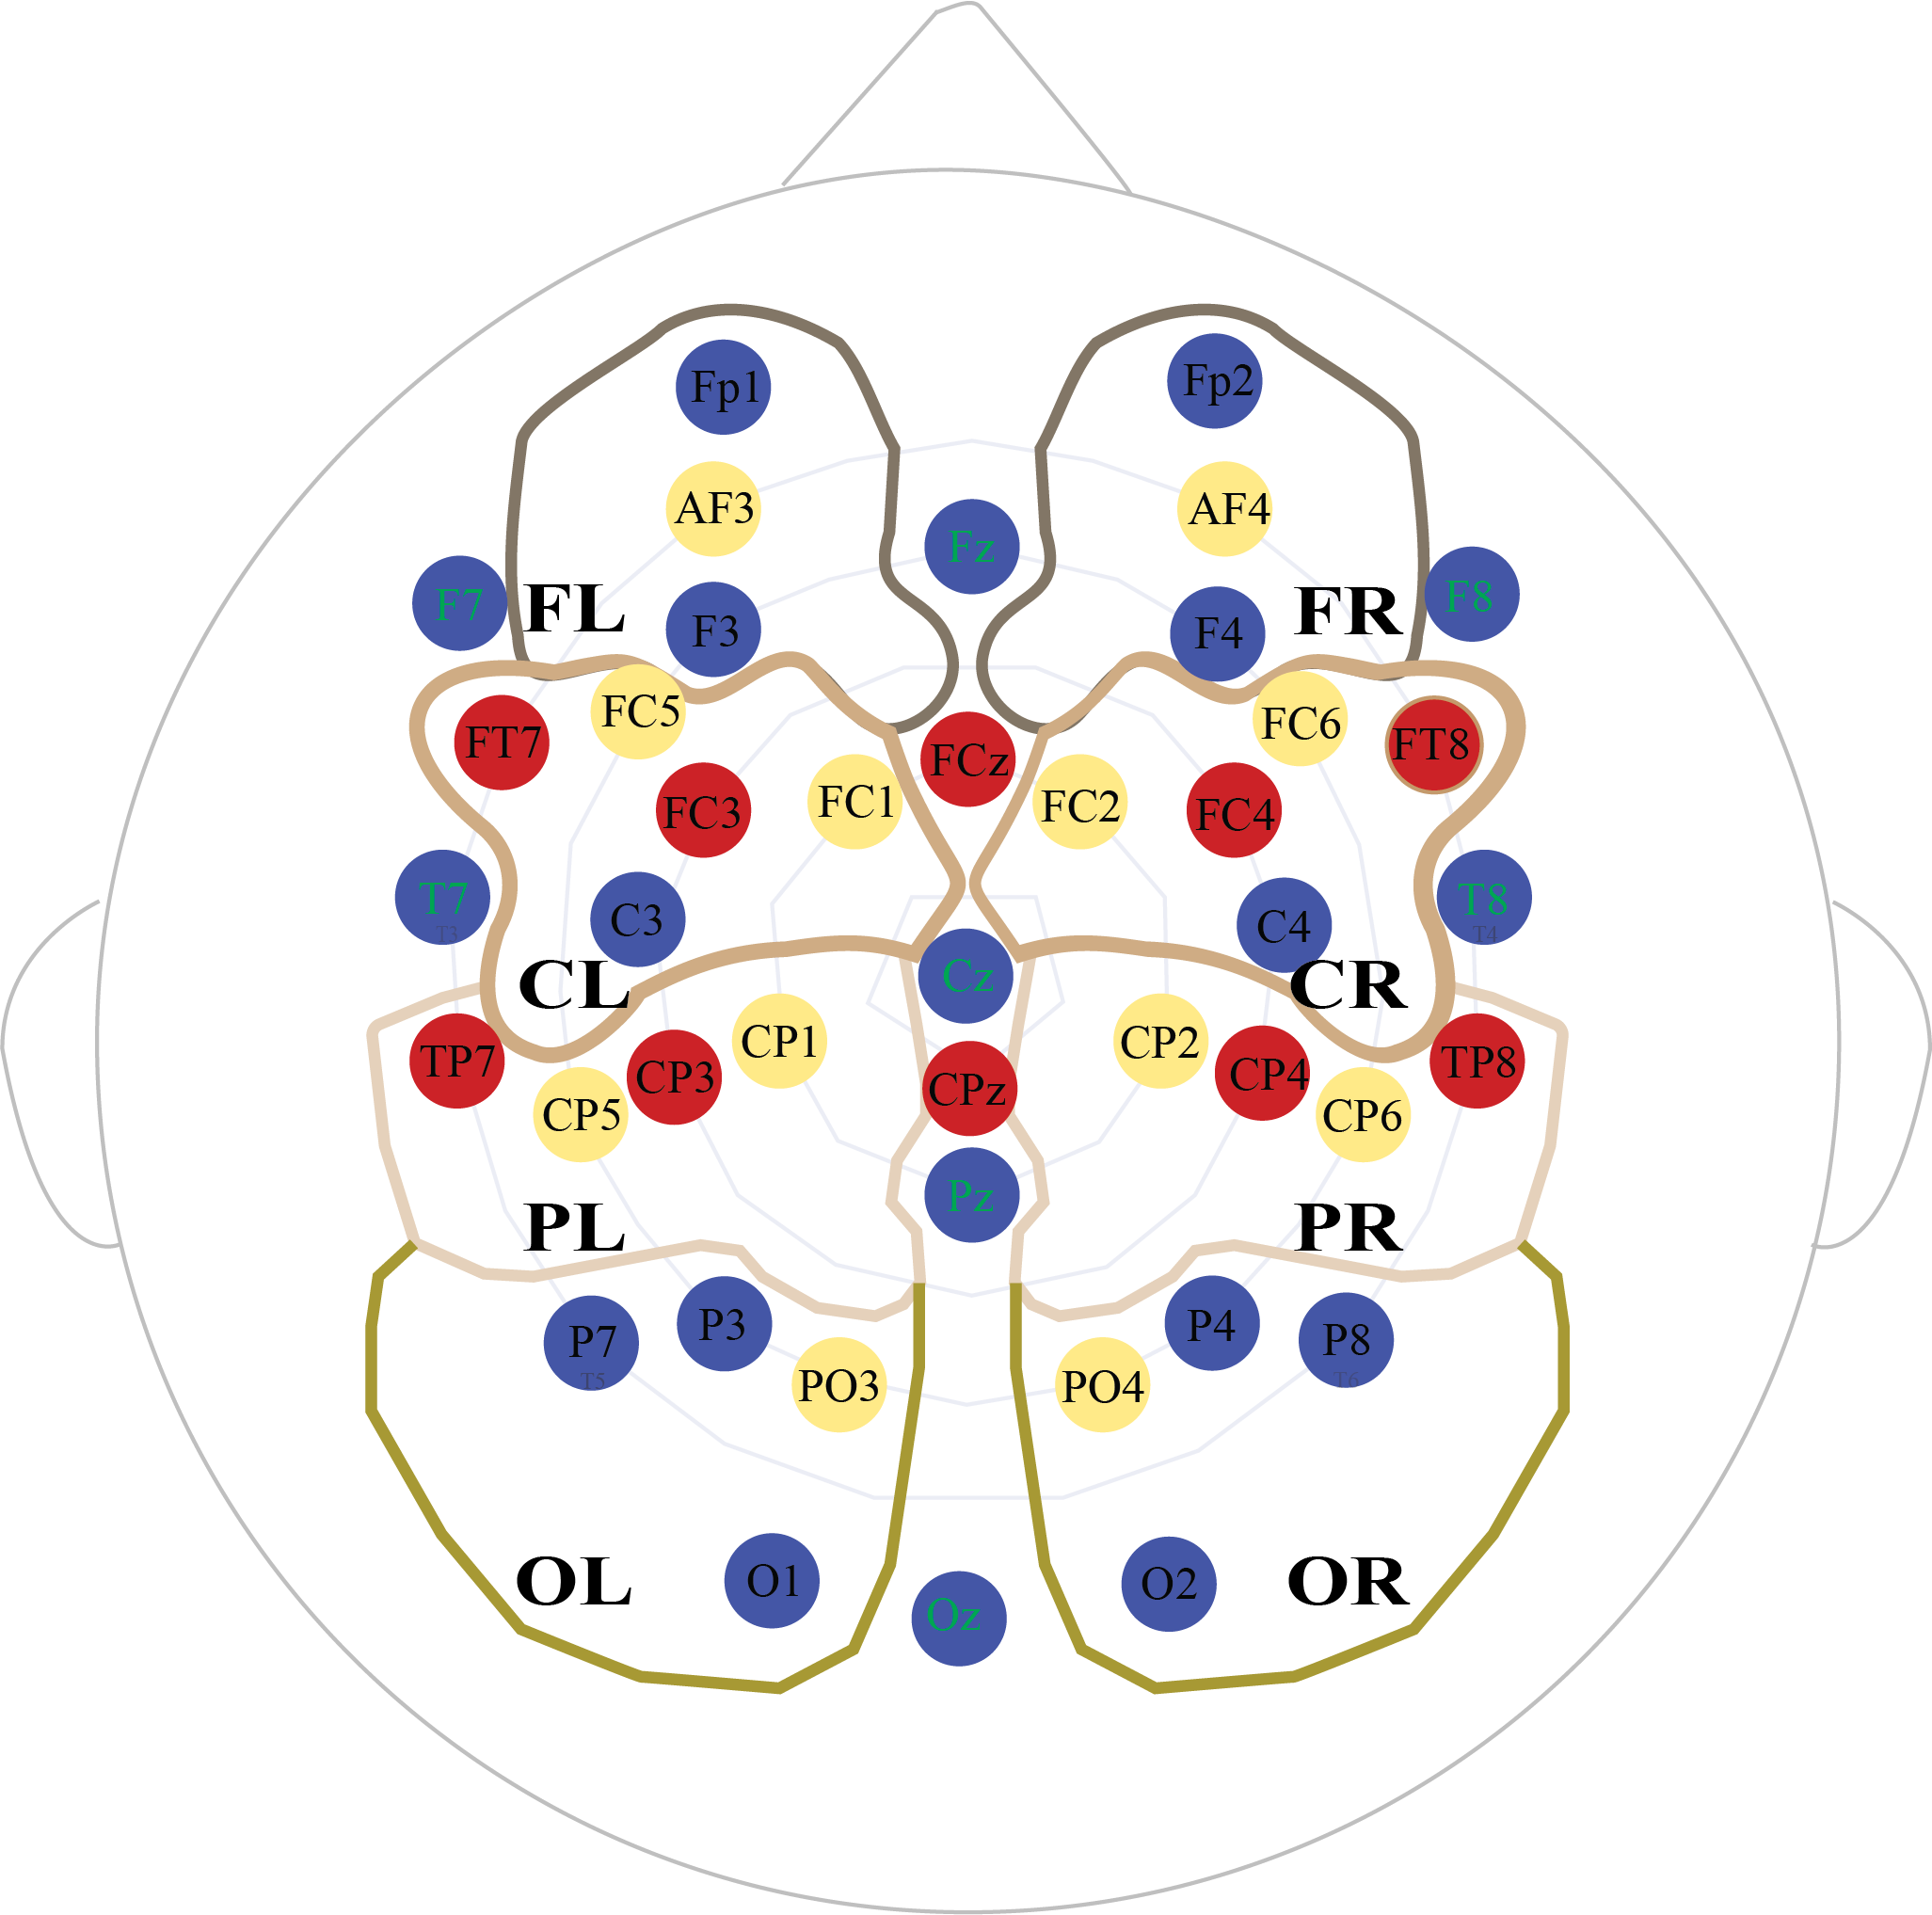
\includegraphics[width=0.9\linewidth]{eeg_map}
    \caption{Scalp locations of the 32 electrodes used in this study, divided into eight anatomical regions (frontal left/right, central left/right, parietal left/right, and occipital left/right, abbreviated FL, FR, CL, CR, PL, PR, OL, and OR). Blue circles mark electrodes present in both the Internal and Cao2018 montages, yellow circles mark electrodes present only in the Internal montage, and red circles mark electrodes present only in the Cao2018 montage.}
    \label{fig:eeg_map}
\end{figure}

\section{Per-Electrode Figures}

Fig.~\ref{fig:exp1_full_montage_per_electrode} shows the per-electrode session-mean $F_1$ when all 32 channels were supplied. On Internal, C3 reached 61.06\% whereas C4 reached only 1.85\%, while on Cao2018 C3 and C4 performed similarly at 31.08\% and 30.18\%, so the C3--C4 asymmetry was specific to Internal. Figs.~\ref{fig:exp1_subset_per_electrode} and~\ref{fig:exp1_subset_per_electrode_stats} show the regional reruns and their comparison with the full montage, and Fig.~\ref{fig:exp1_single_channel} shows the single-electrode runs.

\begin{figure}[ht]
    \centering
    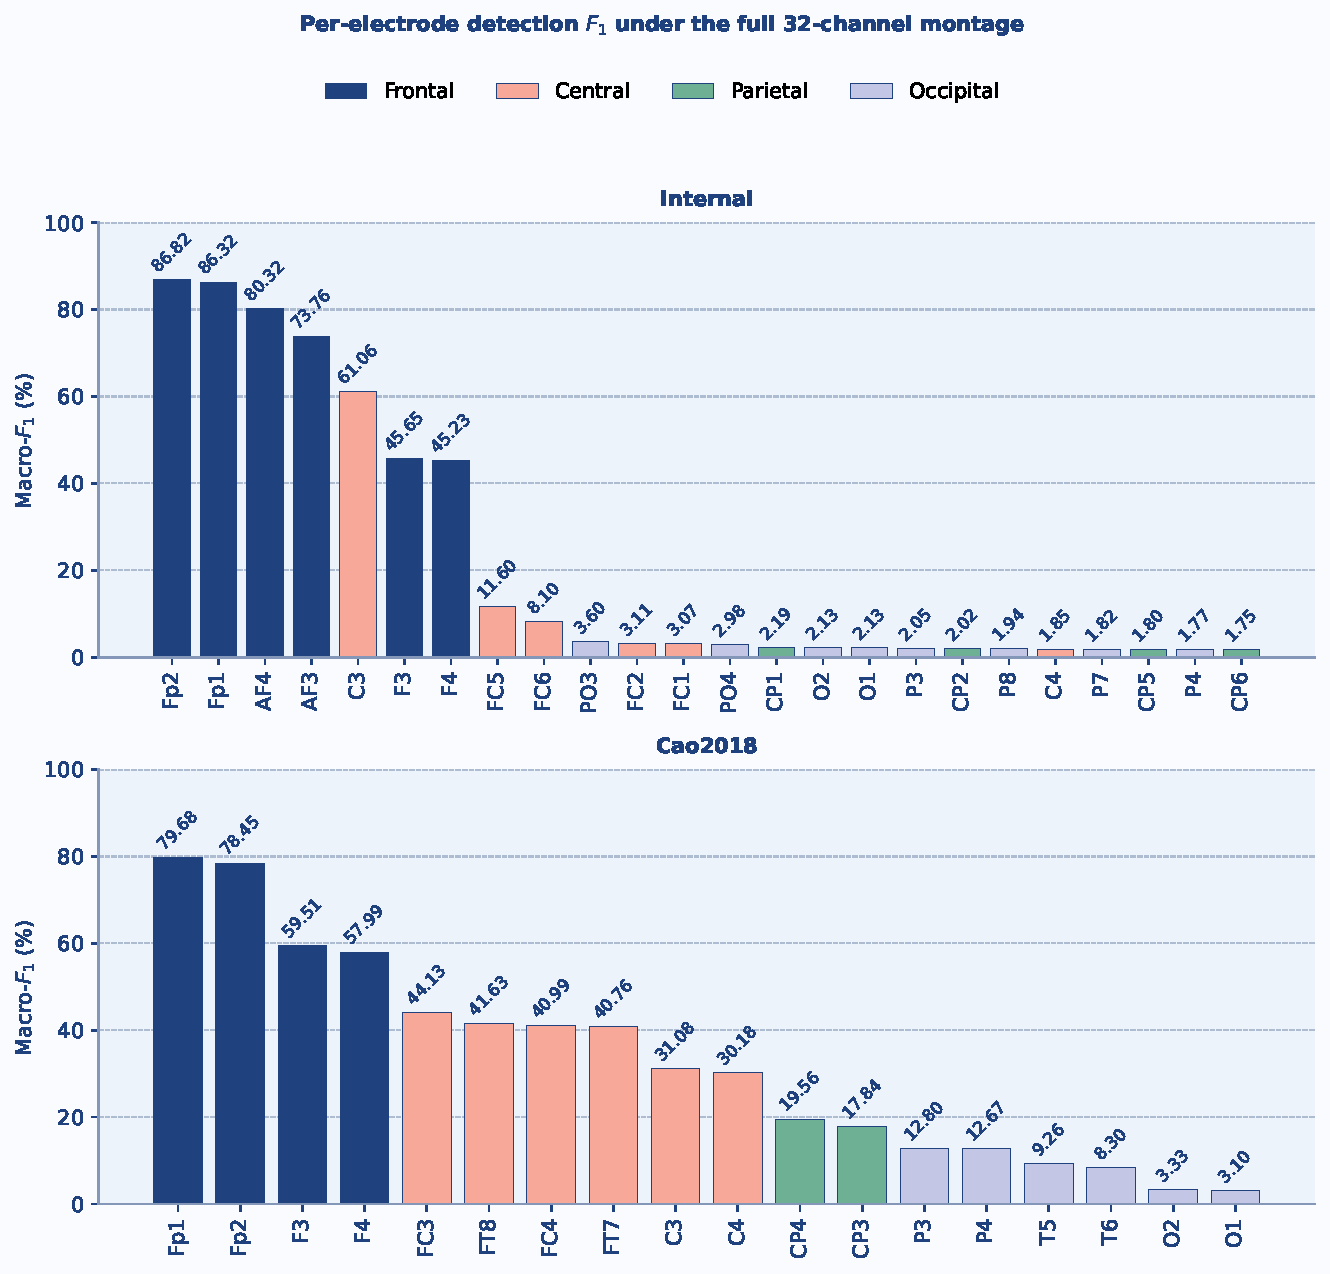
\includegraphics[width=0.9\linewidth]{fig_exp1_full_montage_per_electrode.pdf}
    \caption{Per-electrode detection $F_1$ for every electrode in the four curated anatomical regions, scored in the full-montage run, coloured by scalp region. Each bar is one electrode's session-mean $F_1$ under the complete pipeline using all 32 channels.}
    \label{fig:exp1_full_montage_per_electrode}
\end{figure}

\begin{figure}[ht]
    \centering
    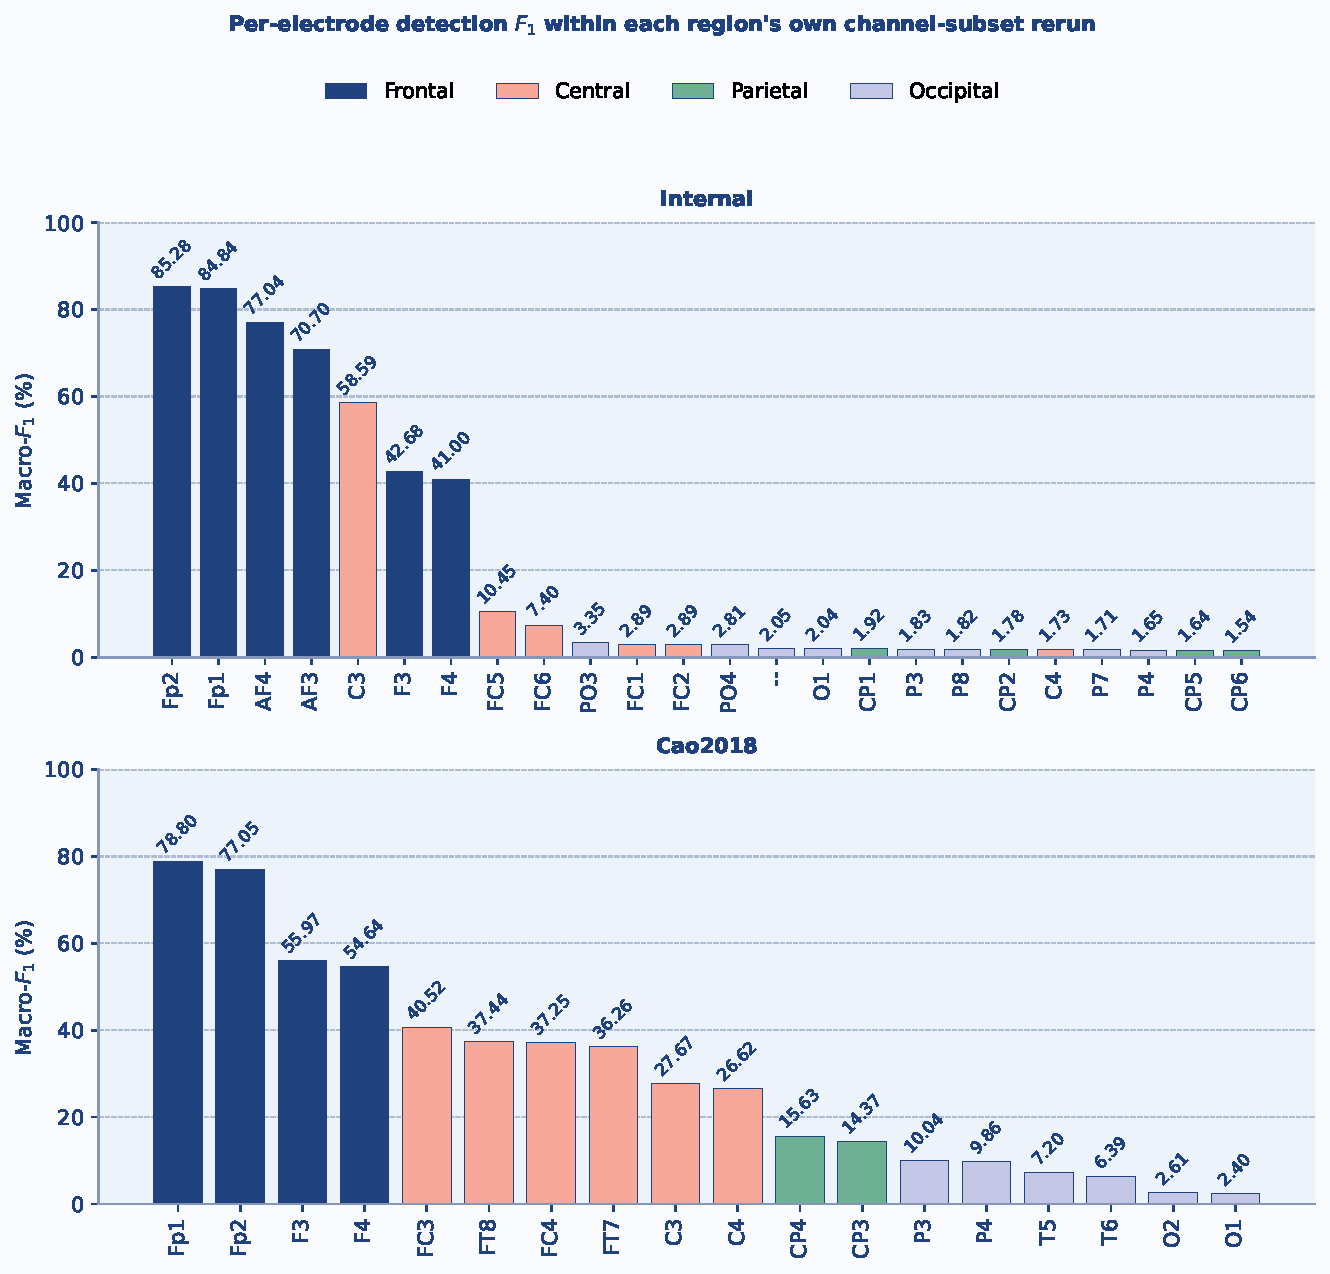
\includegraphics[width=0.9\linewidth]{fig_exp1_subset_per_electrode.pdf}
    \caption{Per-electrode detection $F_1$ in the regional rerun of each electrode's own region, coloured by region. Each bar is one electrode's session-mean $F_1$ when only the electrodes of its region were supplied to the pipeline.}
    \label{fig:exp1_subset_per_electrode}
\end{figure}

\begin{figure}[ht]
    \centering
    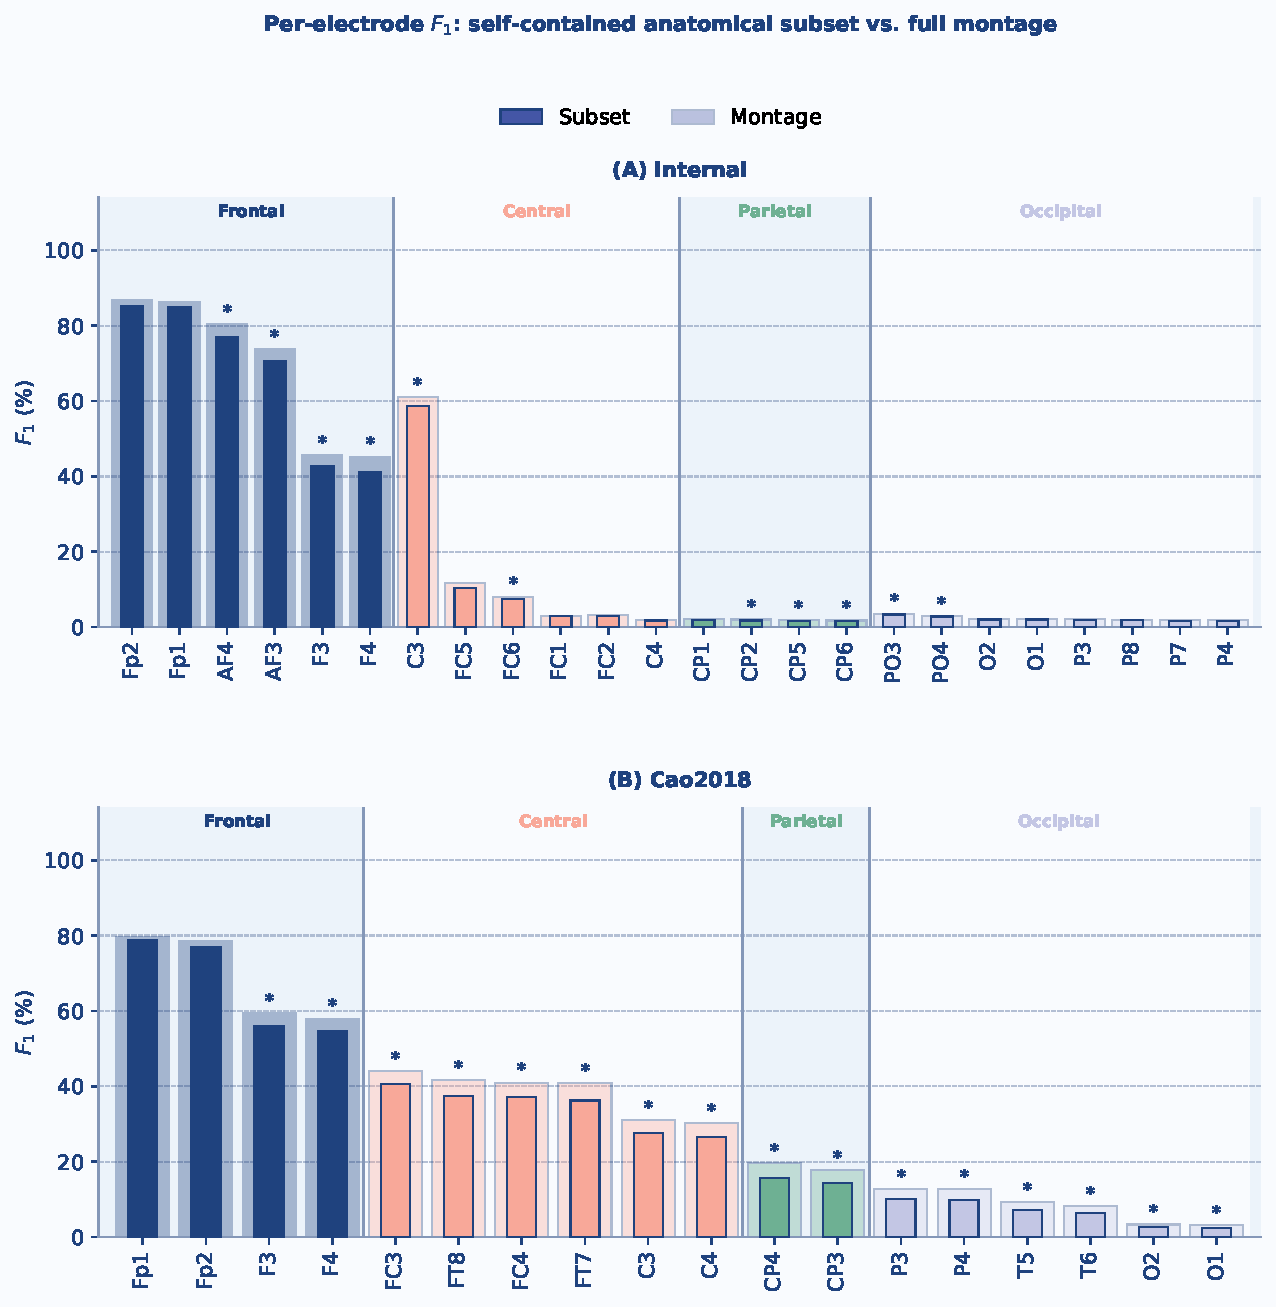
\includegraphics[width=\linewidth]{fig_exp1_subset_per_electrode_stats.pdf}
    \caption{Per-electrode comparison of $F_1$ for each electrode in the rerun of its own anatomical region (narrow, opaque bars) and in the full-montage run (wide, translucent bars), for (A)~Internal and (B)~Cao2018. Bars show session-mean $F_1$. Electrodes are grouped by the anatomical regions in Fig.~\ref{fig:eeg_map} and ordered by descending regional-rerun $F_1$ within each region. Comparisons are paired by session using two-tailed Wilcoxon signed-rank tests, with $p$-values Bonferroni-corrected separately over the electrodes tested within each dataset. An asterisk marks adjusted $p < 0.05$.}
    \label{fig:exp1_subset_per_electrode_stats}
\end{figure}

\begin{figure}[ht]
    \centering
    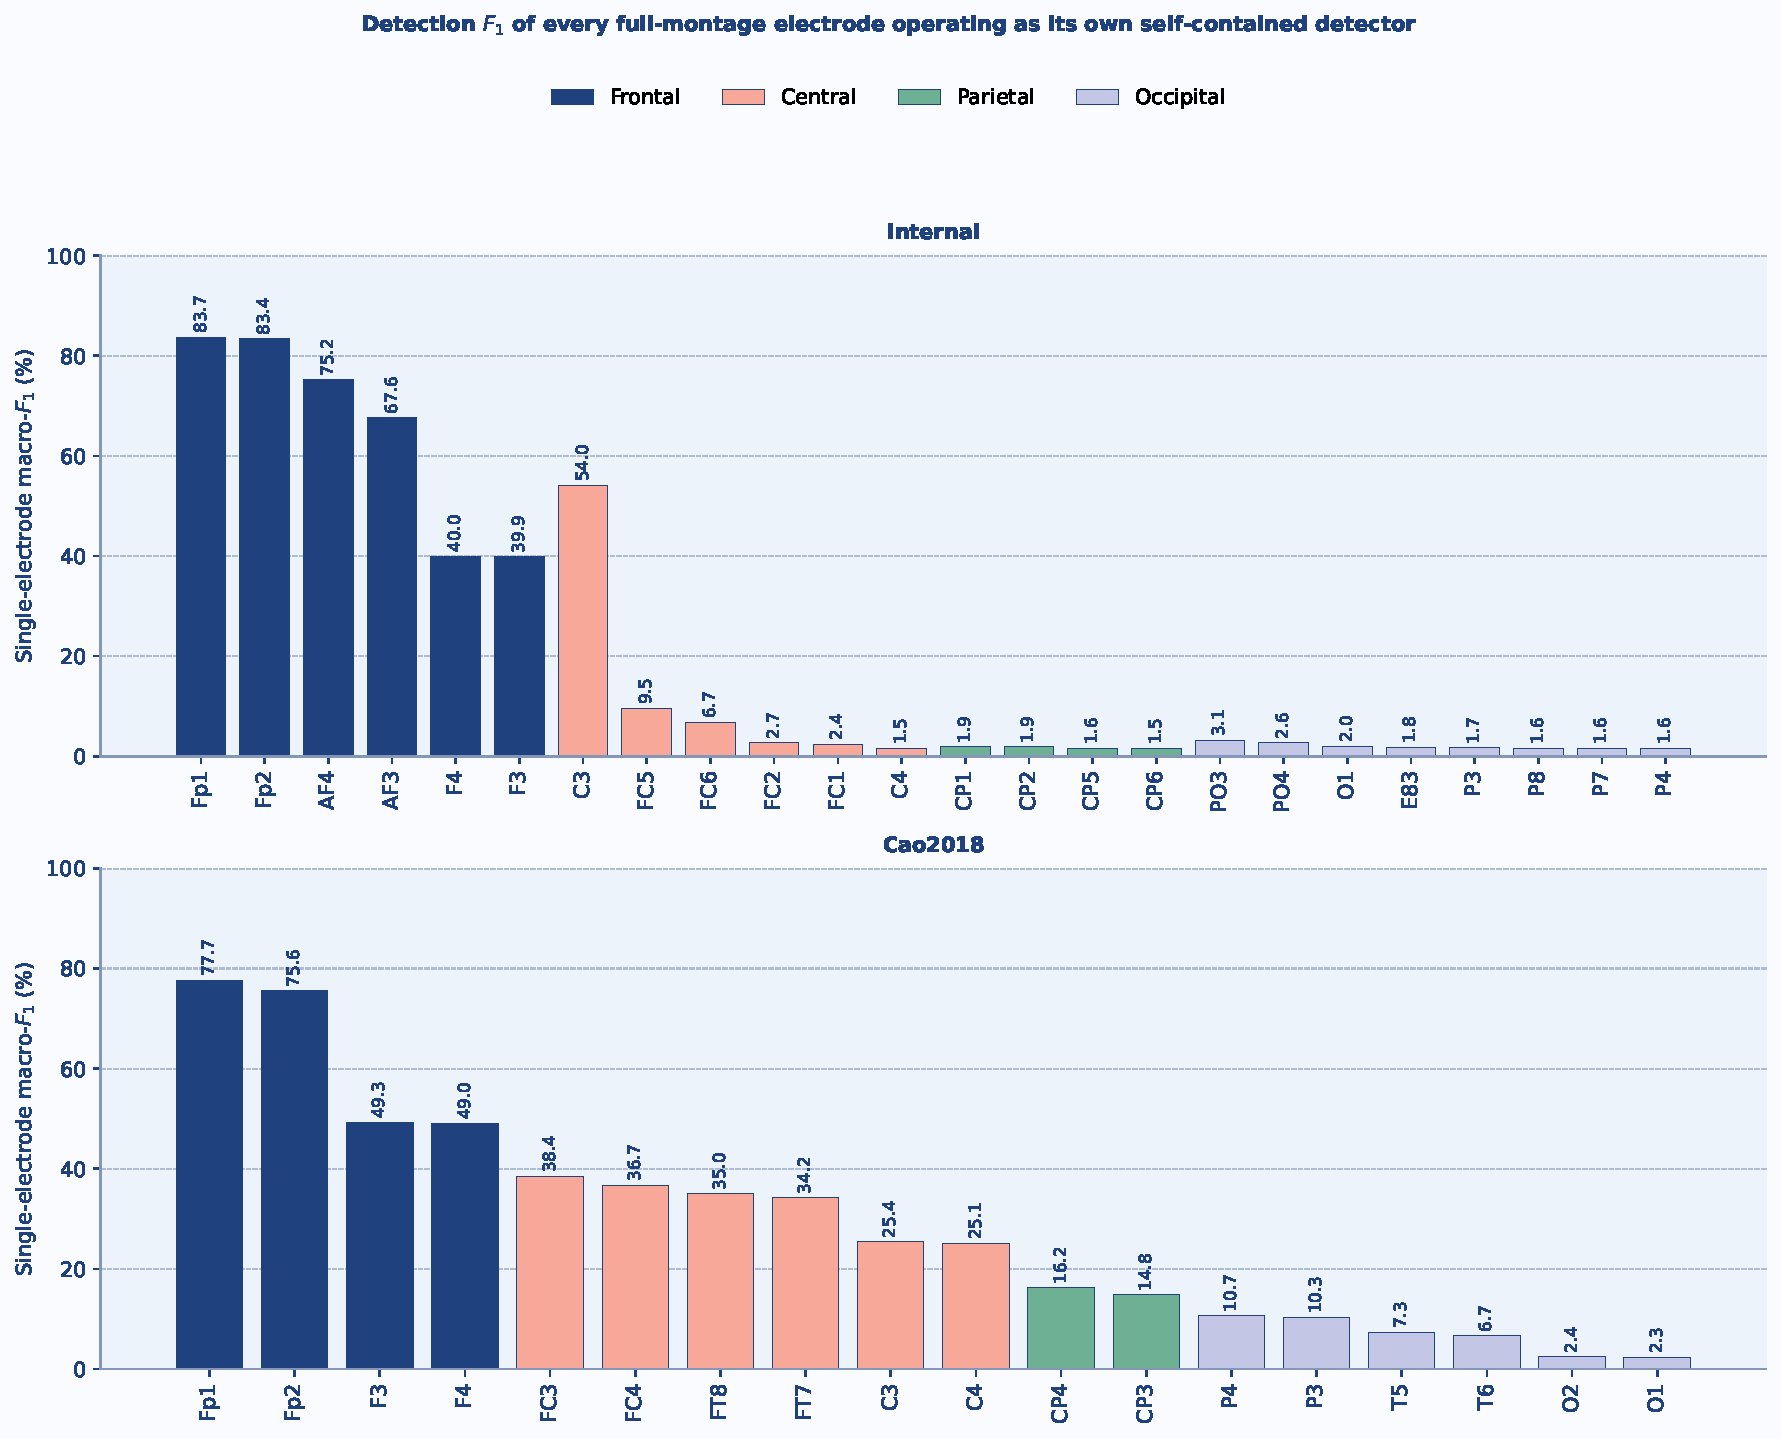
\includegraphics[width=0.9\linewidth]{fig_exp1_single_channel_boxplot.pdf}
    \caption{Detection $F_1$ of every electrode in the four curated anatomical regions operating as its own self-contained detector, in which the complete pipeline was rerun on that one electrode alone, coloured by scalp region.}
    \label{fig:exp1_single_channel}
\end{figure}

\section{Per-Electrode Statistics for the Regional and Single-Electrode Analyses}

Tables~\ref{tab:app_regional_internal} and~\ref{tab:app_regional_cao2018} report, for every electrode, the session-level $F_1$ obtained when the pipeline was rerun with only the electrodes of that electrode's region supplied, alongside the $F_1$ of the same electrode in the full-montage run. Tables~\ref{tab:app_single_internal} and~\ref{tab:app_single_cao2018} report the corresponding comparison for the single-electrode runs, in which each electrode was supplied alone.

\begin{table}[htbp]
  \centering
  \renewcommand{\baselinestretch}{1}\normalsize
  \caption{Per-electrode $F_1$ in the regional rerun versus the full-montage run on the Internal dataset. Each electrode's session-level $F_1$ in the regional rerun, in which only the electrodes of that electrode's region were supplied to the pipeline, was paired with its session-level $F_1$ in the full-montage run (all 32 channels supplied) on the sessions common to both runs and compared with a two-tailed Wilcoxon signed-rank test paired by session. An asterisk ($*$) marks electrodes whose difference was significant at the 0.05 level after Bonferroni correction over the 24 electrodes tested within the Internal dataset. $\Delta F_1$ is the reduced-configuration $F_1$ minus the full-montage $F_1$, in percentage points, so negative values indicate lower $F_1$ in the reduced configuration. Within each region, electrodes are ordered by descending regional-rerun $F_1$.}
  \label{tab:app_regional_internal}
  \footnotesize
  \setlength{\tabcolsep}{2.5pt}
  \begin{tabular}{@{}llrrrc@{}}
    \toprule
     &  & $F_1$ regional & $F_1$ full &  & \\
    Region & Electrode & rerun (\%) & montage (\%) & $\Delta F_1$ & Sig. \\
    \midrule
    Frontal & Fp2 & 85.28 & 86.82 & $-1.54$ & \\
     & Fp1 & 84.84 & 86.32 & $-1.48$ & \\
     & AF4 & 77.04 & 80.32 & $-3.28$ & $*$ \\
     & AF3 & 70.70 & 73.76 & $-3.06$ & $*$ \\
     & F3 & 42.68 & 45.65 & $-2.96$ & $*$ \\
     & F4 & 41.00 & 45.23 & $-4.24$ & $*$ \\
    \addlinespace
    Central & C3 & 58.59 & 61.06 & $-2.47$ & $*$ \\
     & FC5 & 10.45 & 11.60 & $-1.14$ & \\
     & FC6 & 7.40 & 8.10 & $-0.71$ & $*$ \\
     & FC1 & 2.89 & 3.07 & $-0.18$ & \\
     & FC2 & 2.89 & 3.11 & $-0.22$ & \\
     & C4 & 1.73 & 1.85 & $-0.12$ & \\
    \addlinespace
    Parietal & CP1 & 1.92 & 2.19 & $-0.27$ & \\
     & CP2 & 1.78 & 2.02 & $-0.24$ & $*$ \\
     & CP5 & 1.64 & 1.80 & $-0.16$ & $*$ \\
     & CP6 & 1.54 & 1.75 & $-0.20$ & $*$ \\
    \addlinespace
    Occipital & PO3 & 3.35 & 3.60 & $-0.25$ & $*$ \\
     & PO4 & 2.81 & 2.98 & $-0.17$ & $*$ \\
     & O2 & 2.05 & 2.13 & $-0.09$ & \\
     & O1 & 2.04 & 2.13 & $-0.09$ & \\
     & P3 & 1.83 & 2.05 & $-0.22$ & \\
     & P8 & 1.82 & 1.94 & $-0.12$ & \\
     & P7 & 1.71 & 1.82 & $-0.11$ & \\
     & P4 & 1.65 & 1.77 & $-0.12$ & \\
    \bottomrule
  \end{tabular}
\end{table}

\begin{table}[htbp]
  \centering
  \renewcommand{\baselinestretch}{1}\normalsize
  \caption{Per-electrode $F_1$ in the regional rerun versus the full-montage run on the Cao2018 dataset. Each electrode's session-level $F_1$ in the regional rerun, in which only the electrodes of that electrode's region were supplied to the pipeline, was paired with its session-level $F_1$ in the full-montage run (all 32 channels supplied) on the sessions common to both runs and compared with a two-tailed Wilcoxon signed-rank test paired by session. An asterisk ($*$) marks electrodes whose difference was significant at the 0.05 level after Bonferroni correction over the 18 electrodes tested within the Cao2018 dataset. $\Delta F_1$ is the reduced-configuration $F_1$ minus the full-montage $F_1$, in percentage points, so negative values indicate lower $F_1$ in the reduced configuration. Within each region, electrodes are ordered by descending regional-rerun $F_1$.}
  \label{tab:app_regional_cao2018}
  \footnotesize
  \setlength{\tabcolsep}{2.5pt}
  \begin{tabular}{@{}llrrrc@{}}
    \toprule
     &  & $F_1$ regional & $F_1$ full &  & \\
    Region & Electrode & rerun (\%) & montage (\%) & $\Delta F_1$ & Sig. \\
    \midrule
    Frontal & Fp1 & 78.80 & 79.68 & $-0.88$ & \\
     & Fp2 & 77.05 & 78.45 & $-1.40$ & \\
     & F3 & 55.97 & 59.51 & $-3.55$ & $*$ \\
     & F4 & 54.64 & 57.99 & $-3.35$ & $*$ \\
    \addlinespace
    Central & FC3 & 40.52 & 44.13 & $-3.61$ & $*$ \\
     & FT8 & 37.44 & 41.63 & $-4.19$ & $*$ \\
     & FC4 & 37.25 & 40.99 & $-3.73$ & $*$ \\
     & FT7 & 36.26 & 40.76 & $-4.49$ & $*$ \\
     & C3 & 27.67 & 31.08 & $-3.42$ & $*$ \\
     & C4 & 26.62 & 30.18 & $-3.56$ & $*$ \\
    \addlinespace
    Parietal & CP4 & 15.63 & 19.56 & $-3.93$ & $*$ \\
     & CP3 & 14.37 & 17.84 & $-3.46$ & $*$ \\
    \addlinespace
    Occipital & P3 & 10.04 & 12.80 & $-2.77$ & $*$ \\
     & P4 & 9.86 & 12.67 & $-2.81$ & $*$ \\
     & T5 & 7.20 & 9.26 & $-2.06$ & $*$ \\
     & T6 & 6.39 & 8.30 & $-1.91$ & $*$ \\
     & O2 & 2.61 & 3.33 & $-0.72$ & $*$ \\
     & O1 & 2.40 & 3.10 & $-0.70$ & $*$ \\
    \bottomrule
  \end{tabular}
\end{table}

\begin{table}[htbp]
  \centering
  \renewcommand{\baselinestretch}{1}\normalsize
  \caption{Per-electrode $F_1$ in the single-electrode run versus the full-montage run on the Internal dataset. Each electrode's session-level $F_1$ in the single-electrode run, in which that electrode alone was supplied to the pipeline, was paired with its session-level $F_1$ in the full-montage run (all 32 channels supplied) on the sessions common to both runs and compared with a two-tailed Wilcoxon signed-rank test paired by session. An asterisk ($*$) marks electrodes whose difference was significant at the 0.05 level after Bonferroni correction over the 24 electrodes tested within the Internal dataset. $\Delta F_1$ is the reduced-configuration $F_1$ minus the full-montage $F_1$, in percentage points, so negative values indicate lower $F_1$ in the reduced configuration. Within each region, electrodes are ordered by descending single-electrode-run $F_1$.}
  \label{tab:app_single_internal}
  \footnotesize
  \setlength{\tabcolsep}{2.5pt}
  \begin{tabular}{@{}llrrrc@{}}
    \toprule
     &  & $F_1$ single- & $F_1$ full &  & \\
    Region & Electrode & electrode (\%) & montage (\%) & $\Delta F_1$ & Sig. \\
    \midrule
    Frontal & Fp1 & 83.73 & 86.32 & $-2.59$ & \\
     & Fp2 & 83.37 & 86.82 & $-3.45$ & \\
     & AF4 & 75.16 & 80.32 & $-5.16$ & $*$ \\
     & AF3 & 67.59 & 73.76 & $-6.17$ & $*$ \\
     & F4 & 39.98 & 45.23 & $-5.26$ & $*$ \\
     & F3 & 39.85 & 45.65 & $-5.79$ & $*$ \\
    \addlinespace
    Central & C3 & 54.05 & 61.06 & $-7.02$ & $*$ \\
     & FC5 & 9.51 & 11.60 & $-2.09$ & $*$ \\
     & FC6 & 6.73 & 8.10 & $-1.37$ & \\
     & FC2 & 2.69 & 3.11 & $-0.42$ & \\
     & FC1 & 2.42 & 3.07 & $-0.65$ & \\
     & C4 & 1.51 & 1.85 & $-0.34$ & $*$ \\
    \addlinespace
    Parietal & CP1 & 1.86 & 2.19 & $-0.32$ & $*$ \\
     & CP2 & 1.86 & 2.02 & $-0.15$ & \\
     & CP5 & 1.57 & 1.80 & $-0.23$ & \\
     & CP6 & 1.53 & 1.75 & $-0.22$ & \\
    \addlinespace
    Occipital & PO3 & 3.15 & 3.60 & $-0.45$ & $*$ \\
     & PO4 & 2.65 & 2.98 & $-0.34$ & $*$ \\
     & O1 & 1.97 & 2.13 & $-0.16$ & \\
     & O2 & 1.78 & 2.13 & $-0.36$ & $*$ \\
     & P3 & 1.66 & 2.05 & $-0.39$ & $*$ \\
     & P8 & 1.62 & 1.94 & $-0.32$ & $*$ \\
     & P7 & 1.61 & 1.82 & $-0.21$ & $*$ \\
     & P4 & 1.57 & 1.77 & $-0.20$ & \\
    \bottomrule
  \end{tabular}
\end{table}

\begin{table}[htbp]
  \centering
  \renewcommand{\baselinestretch}{1}\normalsize
  \caption{Per-electrode $F_1$ in the single-electrode run versus the full-montage run on the Cao2018 dataset. Each electrode's session-level $F_1$ in the single-electrode run, in which that electrode alone was supplied to the pipeline, was paired with its session-level $F_1$ in the full-montage run (all 32 channels supplied) on the sessions common to both runs and compared with a two-tailed Wilcoxon signed-rank test paired by session. An asterisk ($*$) marks electrodes whose difference was significant at the 0.05 level after Bonferroni correction over the 18 electrodes tested within the Cao2018 dataset. $\Delta F_1$ is the reduced-configuration $F_1$ minus the full-montage $F_1$, in percentage points, so negative values indicate lower $F_1$ in the reduced configuration. Within each region, electrodes are ordered by descending single-electrode-run $F_1$.}
  \label{tab:app_single_cao2018}
  \footnotesize
  \setlength{\tabcolsep}{2.5pt}
  \begin{tabular}{@{}llrrrc@{}}
    \toprule
     &  & $F_1$ single- & $F_1$ full &  & \\
    Region & Electrode & electrode (\%) & montage (\%) & $\Delta F_1$ & Sig. \\
    \midrule
    Frontal & Fp1 & 77.65 & 79.68 & $-2.03$ & \\
     & Fp2 & 75.59 & 78.45 & $-2.86$ & \\
     & F3 & 49.30 & 59.51 & $-10.21$ & $*$ \\
     & F4 & 49.03 & 57.99 & $-8.96$ & $*$ \\
    \addlinespace
    Central & FC3 & 38.44 & 44.13 & $-5.70$ & $*$ \\
     & FC4 & 36.72 & 40.99 & $-4.27$ & $*$ \\
     & FT8 & 34.99 & 41.63 & $-6.63$ & $*$ \\
     & FT7 & 34.22 & 40.76 & $-6.54$ & $*$ \\
     & C3 & 25.43 & 31.08 & $-5.66$ & $*$ \\
     & C4 & 25.10 & 30.18 & $-5.08$ & $*$ \\
    \addlinespace
    Parietal & CP4 & 16.22 & 19.56 & $-3.34$ & $*$ \\
     & CP3 & 14.80 & 17.84 & $-3.04$ & $*$ \\
    \addlinespace
    Occipital & P4 & 10.66 & 12.67 & $-2.01$ & $*$ \\
     & P3 & 10.28 & 12.80 & $-2.52$ & $*$ \\
     & T5 & 7.32 & 9.26 & $-1.94$ & $*$ \\
     & T6 & 6.66 & 8.30 & $-1.64$ & $*$ \\
     & O2 & 2.42 & 3.33 & $-0.91$ & $*$ \\
     & O1 & 2.28 & 3.10 & $-0.82$ & $*$ \\
    \bottomrule
  \end{tabular}
\end{table}

\clearpage
\bibliographystyle{IEEEtran}
\bibliography{references}

\end{document}
